\begin{figure}
  \centering
    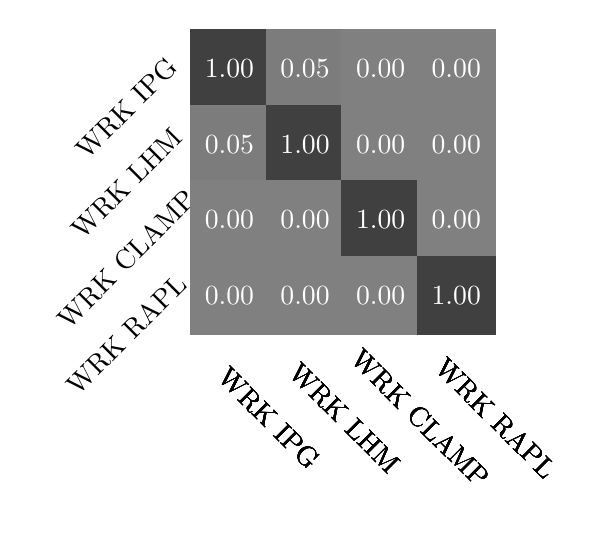
\begin{tikzpicture}[scale=0.6]
      \foreach \y [count=\n] in {{1.00, 0.05, 0.00, 0.00},{0.05, 1.00, 0.00, 0.00},{0.00, 0.00, 1.00, 0.00},{0.00, 0.00, 0.00, 1.00},} {
      % column labels
      \foreach \a [count=\n] in {WRK IPG,WRK LHM,WRK CLAMP,WRK RAPL} {
        \node[minimum size=10mm, xshift=0.5cm, rotate=-45] at (\n*1.6, -9.0) {\a};
      }
      % heatmap tiles
      \foreach \x [count=\m] in \y {
        \pgfmathsetmacro{\xa }{(\x + 1) / 2 * 100}
        \node[fill=darkgray!\xa!lightgray, minimum size=10mm, text=white, font={\normalsize}] at (\m*1.6,-\n*1.6) {\x};
      }
    }
      % row labels
      \foreach \a [count=\i] in {WRK IPG,WRK LHM,WRK CLAMP,WRK RAPL} {
        \node[minimum size=10mm, xshift=-0.35cm, yshift=-0.5cm, rotate=45] at (0,-\i*1.6) {\a};
      }
    \end{tikzpicture}
    \caption{Here the results for the FannkuchRedux on the Mann Whitney U Test can be seen. The Range in $0 - 1$}
    \label{tab:HeatFannkuchRedux2}
\end{figure}